%%%%%%%%%%%%%%%%%%%%%%%%%%%%%%%%%%%%%%%%%%%%%%%%%%%%%%%%%%%%%%%%%%%%%%%%%%%%%%%%
%% 实验报告模板.tex                                              %%
%% author: hxp<hxp201406@gmail.com>                           %%
%% 按照基础物理实验老师发的模板更改形成                                       %%
%%%%%%%%%%%%%%%%%%%%%%%%%%%%%%%%%%%%%%%%%%%%%%%%%%%%%%%%%%%%%%%%%%%%%%%%%%%%%%%%
%% 备注:刚刚的注释刚好是80行,编写代码的时候不要超过80行,就是你的代码不要超 %%
%% 过我注释里面最后面的“%”,超过请换行。                                    %%
%%%%%%%%%%%%%%%%%%%%%%%%%%%%%%%%%%%%%%%%%%%%%%%%%%%%%%%%%%%%%%%%%%%%%%%%%%%%%%%%
%% 模板现在开始,请根据注释把相应的位置更改成对应的内容                       %%
%%%%%%%%%%%%%%%%%%%%%%%%%%%%%%%%%%%%%%%%%%%%%%%%%%%%%%%%%%%%%%%%%%%%%%%%%%%%%%%%


\documentclass{ctexart}

\usepackage{ctex}
\usepackage{amsmath}
\usepackage{amsfonts}
\usepackage{amssymb}
\usepackage{wasysym}
\newcommand{\angstrom}{\text{\normalfont\AA}}  % 定义了原子物理的A
\usepackage{graphicx}
\usepackage{float}
\restylefloat{table}
\usepackage{geometry}
\geometry{a4paper,scale=0.8}  % 定义页面大小是A4,缩放是0.8
\usepackage{caption}
\usepackage{subcaption}
\usepackage{enumitem}
\usepackage{pdfpages}

\newcommand*{\md}{\mathop{}\!\mathrm{d}}   % 定义微分算子,直立体的d
\newcommand*{\me}{\mathrm{e}}              % 定义自然对数e,同样应当是直立体

% 如果你想要每一段的开头不要空两格,注释掉下面这两行
\usepackage{parskip}
\setlength{\parindent}{0cm}

% 默认的\mathbf对希腊字母不生效,这里改下
\usepackage{bm}
\let\Oldmathbf\mathbf
\renewcommand{\mathbf}[1]{\boldsymbol{\Oldmathbf{#1}}}

% 表格默认格内内容和边框没有留出距离,显示分数的时候,分数的上下会贴到边框上
% 因此我增加了表格内容和边框的最短距离是5像素
\usepackage{cellspace}
\setlength{\cellspacetoplimit}{5pt}
\setlength{\cellspacebottomlimit}{5pt}

% \si命令是用来写单位的,单位需要和之前的数字有一个空格的距离,而且应当直立体
% 用法:5 \si{km/h}
\newcommand{\si}[1]{\  \mathrm{#1}}

% 日期不要显示
\date{}

\usepackage{fancyhdr}
\pagestyle{fancy}
\fancyhf{}
\lhead{本文档TeX源码地址:https://github.com/hxp-plus/Notes/tree/master/Physics-Experiment/实验报告}
\rfoot{第 \thepage 页}
\renewcommand{\headrulewidth}{1pt}
\renewcommand{\footrulewidth}{1pt}

%% 标题三号黑体,作者信息为班级姓名学号
\newcommand{\generatetitle}[6]{\title{\zihao{3}\heiti#1} \author{#2 \quad
    \quad #3 \quad\quad #4 \quad\quad #5 \quad\quad #6} \maketitle\thispagestyle{fancy}}

%% 所有的引言、实验内容与数据处理啥的,用section
\ctexset {
  section = {
    format = \raggedright\zihao{4}\heiti,  % 设置所有section的字号为四号黑体左对齐
    name={,、},                            % 序号后跟顿号
    aftername={\hspace{0pt}},              % 修改序号和标题直接的间距为零
    number=\chinese{section},              % 设置序号为中文
  },
  subsection = {
    format = \raggedright\zihao{5}\heiti,  % 设置所有subsection的字号为五号黑体左对齐
    number={},              % 设置序号为没有序号
  },
  subsubsection = {
    format = \raggedright\zihao{5}\heiti,  % 设置所有subsection的字号为五号黑体左对齐
    number={},              % 设置序号为没有序号
  }
}

%% 实验背景、实验目的啥的,用subsection
\ctexset {
  subsection = {
    format = \raggedright\zihao{5}\heiti,  % 所有subsection的字号为五号黑体左对齐
    number={},                             % 设置序号为没有序号
  }
}

%% 把subsection之间加上中括号
\let\oldsubsection\subsection
\renewcommand{\subsection}[1]{\oldsubsection{\!\!\!\!\!\!【#1】}}
\let\oldsubsubsection\subsubsection
\renewcommand{\subsubsection}[1]{\oldsubsubsection{\!\!\!\!\!\!【#1】}}

%% 摘要和关键词用paragraph

\ctexset {
  paragraph = {
    format = \raggedright\zihao{5}\heiti,  % 所有paragraph的字号为五号黑体左对齐
    number={},                             % 设置序号为没有序号
  }
}

%% 把paragraph之间加上中括号
\let\oldparagraph\paragraph
\renewcommand{\paragraph}[1]{\oldparagraph{#1:\!\!\!\!\!\!}}

%% 再把参考文献的序号去掉
\makeatletter
\renewcommand\@biblabel[1]{}
\makeatother

\begin{document}

\generatetitle{综合物理实验报告——
  LabVIEW使用基础}{物理4+4}{胡喜平}{U201811966}{hxp201406@gmail.com}{https://hxp.plus/}

\paragraph{摘要}
本实验学习使用LabVIEW虚拟仪器测量铁的磁滞回线,用采集卡对虚拟仪器进行编程,绘制磁滞回线。

% 关键词
\paragraph{关键词}
虚拟仪器、LabVIEW、磁滞回线

\section{实验原理}
\subsection{铁材料的磁滞现象}

将一个未磁化的铁放入磁场中进行磁化,初次磁化时磁感应强度和磁场的关系是曲线$\overline{ao}$,但是当磁场减为零后,铁内部的磁感应强度没有消失,磁感应强度和磁场强度的曲线是$\overline{ac}$,当磁场强度为零时,磁感应强度是$B_r$,当磁场强度为$-H_C$时,磁感应强度才降为零。
\begin{figure}[H]
  \centering
  \begin{subfigure}{0.48\linewidth}
    \includegraphics[width=\linewidth]{figures/磁滞现象1}
    \subcaption{单条磁滞回线}
  \end{subfigure}
  \begin{subfigure}{0.48\linewidth}
    \includegraphics[width=\linewidth]{figures/磁滞现象2}
    \subcaption{一系列逐渐增大的磁滞回线}
  \end{subfigure}
  \caption{铁材料的磁滞现象}
\end{figure}

反复变化磁场,从$H_m$变化到$-H_m$,刚开始令$H_m$很小,之后逐渐增大$H_m$,可以发现磁化曲线越来越大,直到$H_m$足够大使得铁磁材料处于饱和状态。

\subsection{测量磁滞回线的实验装置原理}

下图是磁滞回线实验装置的原理图,用信号发生器给线圈加入变化的电流,从而产生变化的磁场。铁磁质里面的变化的磁感应强度产生电流,我们测量电流来测量铁磁质中的磁感应强度变化,之后积分得出铁磁质中的磁感应强度。

\begin{figure}[H]
  \centering
  \begin{subfigure}{0.38\linewidth}
    \includegraphics[width=\linewidth]{figures/磁滞回线装置-线圈}
    \subcaption{装置的线圈}
  \end{subfigure}
  \begin{subfigure}{0.58\linewidth}
    \includegraphics[width=\linewidth]{figures/磁滞回线装置-测量电路}
    \subcaption{测量实验结果的电路}
  \end{subfigure}
  \caption{磁滞回线测量实验装置}
\end{figure}

图中左边是输入右边是输出,分别用下标1和2表示。线圈有效长度为$L$,线圈匝数为$N_1$和$N_2$,线圈截面积$A$。

当信号发生器输入的电压产生的交变电流为$i_1$时,产生的磁场为

\begin{equation*}
  \begin{aligned}
    H = \frac{N_1 i_1}{L}
  \end{aligned}
\end{equation*}

其中产生的交变电流通过测量$R$两端的电压间接得到。产生的磁感应强度需要通过积分得到

\begin{equation*}
  \begin{aligned}
    B = \int \frac{v\md t}{N_2 A}
  \end{aligned}
\end{equation*}

其中$v$是感应电压。

\section{实验内容}

用LabVIEW虚拟仪器测量材料的磁滞现象和磁滞回线。

\section{实验结果的分析和结论}

\subsection{信号测量系统测试}

\subsubsection{模拟输入}

用信号发生器输出50Hz,幅度为8V的正弦波,输入信号的示波器测量结果和采集卡测量结果如下

\begin{figure}[H]
  \centering
  \begin{subfigure}{0.41\linewidth}
    \includegraphics[width=\linewidth]{LabVIEW使用基础/信号测量系统测试/模拟输入/正弦波/示波器.JPG}
    \subcaption{输入信号示波器测量结果}
  \end{subfigure}
  \begin{subfigure}{0.54\linewidth}
    \includegraphics[width=\linewidth]{LabVIEW使用基础/信号测量系统测试/模拟输入/正弦波/虚拟仪器.PNG}
    \subcaption{虚拟仪器采集卡得到的结果}
  \end{subfigure}
  \caption{正弦信号,幅度8V,50Hz}
\end{figure}

用信号发生器输出50Hz,幅度为8V,占空比30\%的方波,输入信号的示波器测量结果和采集卡测量结果如下

\begin{figure}[H]
  \centering
  \begin{subfigure}{0.41\linewidth}
    \includegraphics[width=\linewidth]{LabVIEW使用基础/信号测量系统测试/模拟输入/方波/示波器.JPG}
    \subcaption{输入信号示波器测量结果}
  \end{subfigure}
  \begin{subfigure}{0.54\linewidth}
    \includegraphics[width=\linewidth]{LabVIEW使用基础/信号测量系统测试/模拟输入/方波/虚拟仪器_采样率1000.PNG}
    \subcaption{虚拟仪器采集卡得到的结果,采样率1000}
  \end{subfigure}
  \caption{方波信号,幅度8V,50Hz,占空比30\%}
\end{figure}

后来更换了采集卡的采样率

\begin{figure}[H]
  \centering
  \begin{subfigure}{0.48\linewidth}
    \includegraphics[width=\linewidth]{LabVIEW使用基础/信号测量系统测试/模拟输入/方波/虚拟仪器_采样率500.PNG}
    \subcaption{虚拟仪器采集卡得到的结果,采样率500}
  \end{subfigure}
  \begin{subfigure}{0.48\linewidth}
    \includegraphics[width=\linewidth]{LabVIEW使用基础/信号测量系统测试/模拟输入/方波/虚拟仪器_采样率2000.PNG}
    \subcaption{虚拟仪器采集卡得到的结果,采样率2000}
  \end{subfigure}
  \caption{方波信号,幅度8V,50Hz,占空比30\%}
\end{figure}

发现如果是方波这种变化比较大的波,采样率如果太低,那采集的图像失真会比较严重。

\subsubsection{模拟输出}

另采集卡输出直流和正弦波信号,用示波器测量输出信号

\begin{figure}[H]
  \centering
  \begin{subfigure}{0.54\linewidth}
    \includegraphics[width=\linewidth]{LabVIEW使用基础/信号测量系统测试/模拟输出/方波/虚拟仪器.PNG}
    \subcaption{虚拟仪器输出信号参数,直流}
  \end{subfigure}
  \begin{subfigure}{0.41\linewidth}
    \includegraphics[width=\linewidth]{LabVIEW使用基础/信号测量系统测试/模拟输出/方波/示波器.JPG}
    \subcaption{示波器测量得到的图像,直流}
  \end{subfigure}
  \begin{subfigure}{0.54\linewidth}
    \includegraphics[width=\linewidth]{LabVIEW使用基础/信号测量系统测试/模拟输出/正弦波/虚拟仪器.PNG}
    \subcaption{虚拟仪器输出信号参数,正弦波}
  \end{subfigure}
  \begin{subfigure}{0.41\linewidth}
    \includegraphics[width=\linewidth]{LabVIEW使用基础/信号测量系统测试/模拟输出/正弦波/示波器.JPG}
    \subcaption{示波器测量得到的图像,正弦波}
  \end{subfigure}
  \caption{模拟输出,直流和正弦波}
\end{figure}

\subsection{模拟信号测量}

用信号发生器输出正弦波、方波,编写程序,在软件界面上显示测量结果。

\begin{figure}[H]
  \centering
  \includegraphics[width=0.98\linewidth]{LabVIEW使用基础/模拟信号测量/程序.PNG}
  \caption{信号测量程序框图}
\end{figure}

\begin{figure}[H]
  \centering
  \begin{subfigure}{0.49\linewidth}
    \includegraphics[width=\linewidth]{LabVIEW使用基础/模拟信号测量/前面板-正弦波.PNG}
    \subcaption{正弦波测量结果}
  \end{subfigure}
  \begin{subfigure}{0.49\linewidth}
    \includegraphics[width=\linewidth]{LabVIEW使用基础/模拟信号测量/前面板-方波.PNG}
    \subcaption{方波测量结果}
  \end{subfigure}
  \caption{程序测量结果}
\end{figure}

\newpage
\subsection{周期电信号的傅里叶分析}

直接使用LabVIEW内置的傅里叶分析程序,测量了方波和三角波

\begin{figure}[H]
  \centering
  \includegraphics[width=0.98\linewidth]{LabVIEW使用基础/周期电信号的傅里叶分析/三角波.PNG}
  \caption{三角波傅里叶分析}
\end{figure}

\begin{figure}[H]
  \centering
  \includegraphics[width=0.98\linewidth]{LabVIEW使用基础/周期电信号的傅里叶分析/方波.PNG}
  \caption{方波傅里叶分析}
\end{figure}

\newpage
\subsection{交流励磁法测量材料的磁导率}

使用的程序如下

\begin{figure}[H]
  \centering
  \includegraphics[width=0.98\linewidth]{LabVIEW使用基础/铁材料的磁滞现象和磁滞回线/测量程序.png}
  \caption{测量磁滞回线的程序框图}
\end{figure}

不断增大信号发生器的电压,以增大励磁电流,获得的图像如下

\begin{figure}[H]
  \centering
  \begin{subfigure}{0.32\linewidth}
    \includegraphics[width=\linewidth]{LabVIEW使用基础/铁材料的磁滞现象和磁滞回线/3V.png}
    \subcaption{信号发生器电压3V}
  \end{subfigure}
  \begin{subfigure}{0.32\linewidth}
    \includegraphics[width=\linewidth]{LabVIEW使用基础/铁材料的磁滞现象和磁滞回线/4V.png}
    \subcaption{信号发生器电压4V}
  \end{subfigure}
  \begin{subfigure}{0.32\linewidth}
    \includegraphics[width=\linewidth]{LabVIEW使用基础/铁材料的磁滞现象和磁滞回线/5V.png}
    \subcaption{信号发生器电压5V}
  \end{subfigure}
  \caption{测量磁滞回线,电压3-5V}
\end{figure}

\begin{figure}[H]
  \centering
  \begin{subfigure}{0.32\linewidth}
    \includegraphics[width=\linewidth]{LabVIEW使用基础/铁材料的磁滞现象和磁滞回线/7V.png}
    \subcaption{信号发生器电压7V}
  \end{subfigure}
  \begin{subfigure}{0.32\linewidth}
    \includegraphics[width=\linewidth]{LabVIEW使用基础/铁材料的磁滞现象和磁滞回线/8V.png}
    \subcaption{信号发生器电压8V}
  \end{subfigure}
  \begin{subfigure}{0.32\linewidth}
    \includegraphics[width=\linewidth]{LabVIEW使用基础/铁材料的磁滞现象和磁滞回线/9V.png}
    \subcaption{信号发生器电压9V}
  \end{subfigure}
  \begin{subfigure}{0.32\linewidth}
    \includegraphics[width=\linewidth]{LabVIEW使用基础/铁材料的磁滞现象和磁滞回线/10V.png}
    \subcaption{信号发生器电压10V}
  \end{subfigure}
  \begin{subfigure}{0.16\linewidth}
    \phantom{}
  \end{subfigure}
  \begin{subfigure}{0.32\linewidth}
    \includegraphics[width=\linewidth]{LabVIEW使用基础/铁材料的磁滞现象和磁滞回线/20V.png}
    \subcaption{信号发生器电压20V}
  \end{subfigure}
  \caption{测量磁滞回线,电压7-20V}
\end{figure}

可以发现,当励磁电流越大,也就是说,当磁场的变化范围越大,磁滞回线现象越明显。选取10V和20V的数据进行了数据处理,绘制的磁场强度和磁导率关系如下

\begin{figure}[H]
  \centering
  \begin{subfigure}{0.48\linewidth}
    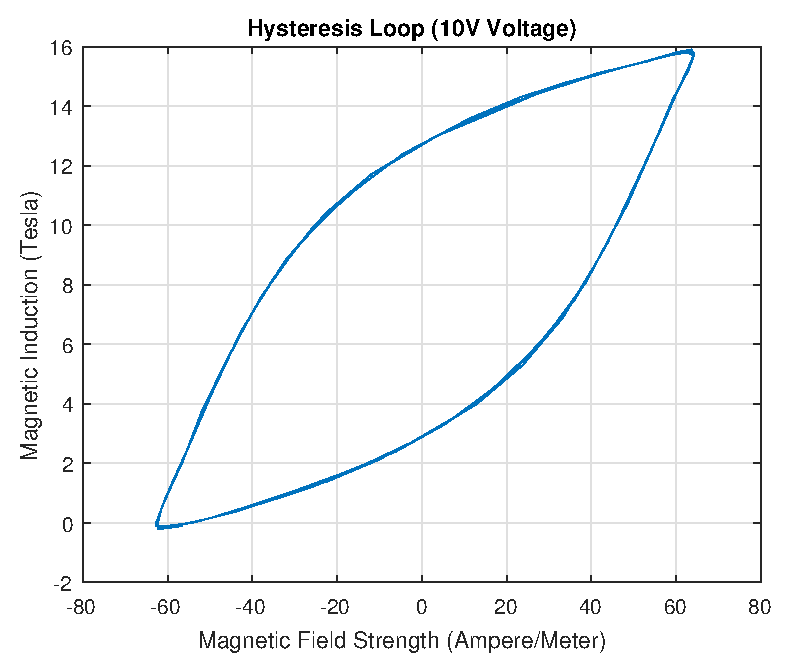
\includegraphics[width=\linewidth]{LabVIEW使用基础/数据处理/HysteresisLoop_10V.eps}
    \subcaption{10V,磁滞回线}
  \end{subfigure}
  \begin{subfigure}{0.48\linewidth}
    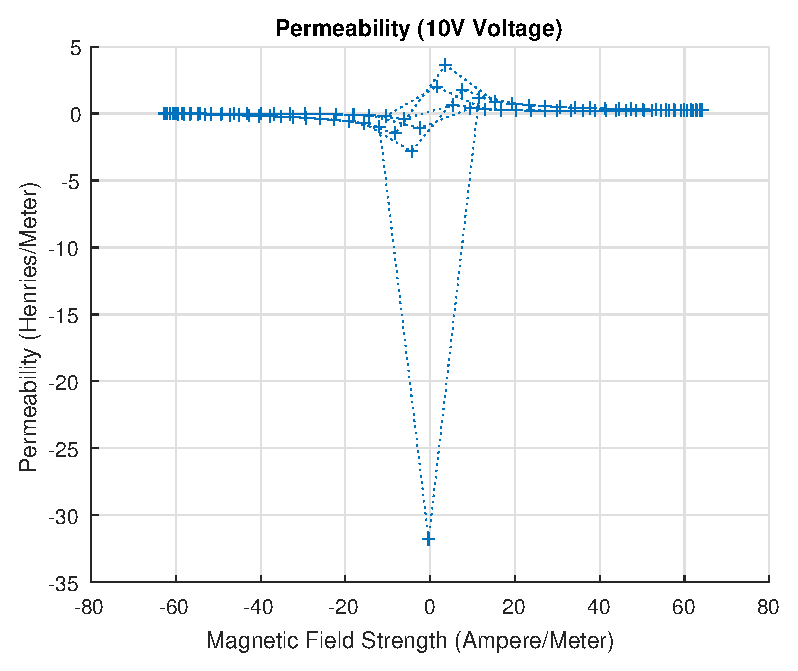
\includegraphics[width=\linewidth]{LabVIEW使用基础/数据处理/Permeability_10V.eps}
    \subcaption{10V,磁导率随磁场变化}
  \end{subfigure}
  \caption{磁滞回线和磁导率随磁场变化图像,10V}
\end{figure}

\begin{figure}[H]
  \centering
  \begin{subfigure}{0.48\linewidth}
    \includegraphics[width=\linewidth]{LabVIEW使用基础/数据处理/HysteresisLoop_20V.eps}
    \subcaption{20V,磁滞回线}
  \end{subfigure}
  \begin{subfigure}{0.48\linewidth}
    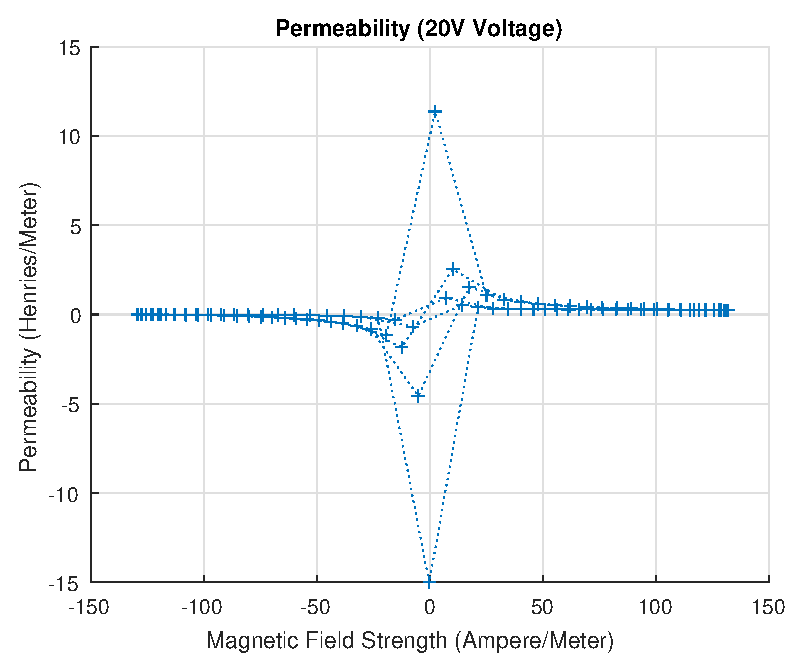
\includegraphics[width=\linewidth]{LabVIEW使用基础/数据处理/Permeability_20V.eps}
    \subcaption{20V,磁导率随磁场变化}
  \end{subfigure}
  \caption{磁滞回线和磁导率随磁场变化图像,20V}
\end{figure}

磁导率曲线应当是磁场增强时从0开始逐渐上升,然后上升到一个最高点后下降到0。磁场反向增加的时候应当是先下降到最低点,然后逐渐上升到0。这两组数据有一点这个趋势,但是不明显。主要是因为采样率选的低了,如果能在磁场从0开始增加的那时候选取更多的采样点,实验的结果就会更符合理论。

\end{document} 

%%% Local Variables:
%%% mode: latex
%%% TeX-master: t
%%% End:
